
\documentclass[journal]{IEEEtran}

% ------------------------------------------------------------
% PLANTILLA - IMT-342 ROBÓTICA
% Primer Parcial Práctico: Cinemática de manipuladores con ROS 2
%
% IMPORTANTE:
% 1) Reemplazar todos los textos entre [CORCHETES].
% 2) Eliminar las cajas "INSTRUCCIÓN" antes de la entrega final,
%    salvo que el docente indique lo contrario.
% 3) No copiar parámetros DH ni resultados de otro grupo.
% 4) El repositorio GitHub debe permitir reproducir el trabajo
%    en otra computadora con Ubuntu 24.04 + ROS 2 Jazzy.
% ------------------------------------------------------------

\usepackage[utf8]{inputenc}
\usepackage[T1]{fontenc}
\usepackage[spanish,es-nodecimaldot]{babel}
\usepackage{graphicx}
\usepackage{amsmath,amssymb}
\usepackage{booktabs}
\usepackage{float}
\usepackage{array}
\usepackage{tabularx}
\usepackage{xcolor}
\usepackage{listings}
\usepackage{enumitem}
\usepackage{hyperref}
\usepackage{url}
\usepackage{siunitx}

\hypersetup{
    colorlinks=true,
    linkcolor=blue,
    urlcolor=blue,
    citecolor=blue
}

\lstset{
    basicstyle=\ttfamily\footnotesize,
    breaklines=true,
    frame=single,
    columns=fullflexible,
    keepspaces=true
}

\newcommand{\instr}[1]{%
\begin{quote}
\small
\noindent\textbf{\color{blue}{INSTRUCCIÓN:}} #1
\end{quote}
}

\newcommand{\pendiente}[1]{\textbf{\color{red}{[#1]}}}

\title{Primer Parcial Práctico\\
Cinemática Directa e Inversa del Robot KUKA KR 7 R900-3 con ROS 2 Jazzy}

\author{
\textbf{Grupo 7}\\
Yohel Felipe Tancara Poma\\
Jhamil Alexis Gutierrez Huarayo\\
IMT-342 Robótica -- Universidad Católica Boliviana ``San Pablo''\\
Docente: Carlos Daniel Aguilar Mancachi
}

\date{4 de octubre de 2026}

\begin{document}
\maketitle

% ============================================================
\begin{abstract}
\instr{Redactar entre 120 y 180 palabras. Resumir el robot asignado, la obtención de los parámetros Denavit--Hartenberg, el desarrollo de la cinemática directa, el método utilizado para la cinemática inversa, la implementación en ROS 2 y los principales resultados de validación. No incluir citas ni resultados que no aparezcan desarrollados posteriormente.}

\pendiente{REEMPLAZAR POR EL RESUMEN DEL GRUPO.}
\end{abstract}

\begin{IEEEkeywords}
Denavit--Hartenberg, cinemática directa, cinemática inversa, Jacobiano, ROS 2, RViz2, manipulador serial.
\end{IEEEkeywords}

% ============================================================
\section{Requisitos mínimos de la entrega}

\instr{Esta sección funciona como lista de control. Puede mantenerse en el borrador y eliminarse en la versión final. El informe debe demostrar desarrollo matemático propio y validación en ROS 2.}

La entrega del Primer Parcial Práctico debe contener, como mínimo:

\begin{enumerate}[leftmargin=*]
    \item Identificación completa del robot asignado y de su cadena cinemática.
    \item Asignación justificada de marcos de referencia.
    \item Tabla completa de parámetros Denavit--Hartenberg.
    \item Matriz homogénea general y matrices particulares de cada transformación.
    \item Cinemática directa simbólica y/o semisimbólica.
    \item Obtención de la posición y orientación del efector final.
    \item Desarrollo del Jacobiano posicional empleado en la cinemática inversa.
    \item Formulación e implementación de la cinemática inversa de posición para un objetivo cartesiano $(x,y,z)$.
    \item Recepción del objetivo mediante el tópico \texttt{/target} con mensajes \texttt{geometry\_msgs/msg/Point}.
    \item Publicación de la solución articular mediante \texttt{/joint\_states}.
    \item Criterio de inicialización, convergencia, tolerancia y límites articulares.
    \item Validación matemática mediante al menos tres configuraciones articulares.
    \item Validación de cinemática inversa mediante al menos tres objetivos alcanzables.
    \item Implementación propia en ROS 2.
    \item Evidencia en RViz2 y Joint State Publisher GUI.
    \item Estructura del workspace y comandos de compilación/ejecución.
    \item Enlace a un repositorio GitHub reproducible.
    \item README del repositorio con instrucciones completas desde una computadora nueva.
    \item Conclusiones técnicas del grupo.
\end{enumerate}

% ============================================================
\section{Descripción del robot asignado}

\instr{Describir únicamente el robot asignado al grupo. Incluir fabricante, modelo, número de grados de libertad utilizados, tipo de articulaciones, alcance aproximado si la fuente oficial lo proporciona y la identificación del marco base y del efector final. Citar la documentación oficial utilizada.}

\subsection{Datos generales}

El robot asignado al Grupo 7 es el KUKA KR 7 R900-3,
perteneciente a la familia de robots industriales de pequeño
tamaño de KUKA. El manipulador dispone de seis grados de
libertad, implementados mediante seis articulaciones revolutas.
De acuerdo con la documentación del fabricante, posee un
alcance máximo aproximado de 902 mm y una capacidad de carga
nominal de 7 kg \cite{robot_docs}.

En el modelo utilizado en ROS 2, la cadena cinemática comienza
en el marco \texttt{base\_link} y se consideran las articulaciones
\texttt{joint\_1} hasta \texttt{joint\_6}. Como marco asociado al
efector final se utiliza \texttt{tool0}. Las magnitudes lineales
se expresan en metros y las variables articulares en radianes.

\begin{table}[H]
\centering
\caption{Datos principales del robot}
\begin{tabular}{ll}
\toprule
\textbf{Dato} & \textbf{Valor} \\
\midrule
Fabricante & KUKA \\
Modelo & KR 7 R900-3 \\
Grados de libertad & 6 \\
Tipo de articulaciones & 6 revolutas \\
Alcance máximo & 0.902 m \\
Carga nominal & 7 kg \\
Marco base & \texttt{base\_link} \\
Efector final & \texttt{tool0} \\
Unidades empleadas & SI: metros y radianes \\
\bottomrule
\end{tabular}
\end{table}

\subsection{Cadena cinemática}

El KUKA KR 7 R900-3 presenta una cadena cinemática serial
compuesta por seis articulaciones revolutas. Cada articulación
conecta de manera sucesiva los eslabones del manipulador,
desde el marco fijo \texttt{base\_link} hasta el efector final
\texttt{tool0}.

La cadena utilizada en el modelo ROS 2 es:

\[
\begin{aligned}
\texttt{base\_link}
&\xrightarrow{q_1}
\texttt{link\_1}
\xrightarrow{q_2}
\texttt{link\_2}
\xrightarrow{q_3}
\texttt{link\_3}
\\[2mm]
\texttt{link\_3}
&\xrightarrow{q_4}
\texttt{link\_4}
\xrightarrow{q_5}
\texttt{link\_5}
\xrightarrow{q_6}
\texttt{link\_6}
\\[2mm]
\texttt{link\_6}
&\rightarrow
\texttt{tool0}.
\end{aligned}
\]

\instr{Insertar una figura del robot donde se distingan claramente las articulaciones $q_1,\dots,q_n$. La imagen puede provenir de la documentación oficial o ser una captura propia de RViz2, pero debe citarse o identificarse correctamente.}

\begin{figure}[H]
    \centering
    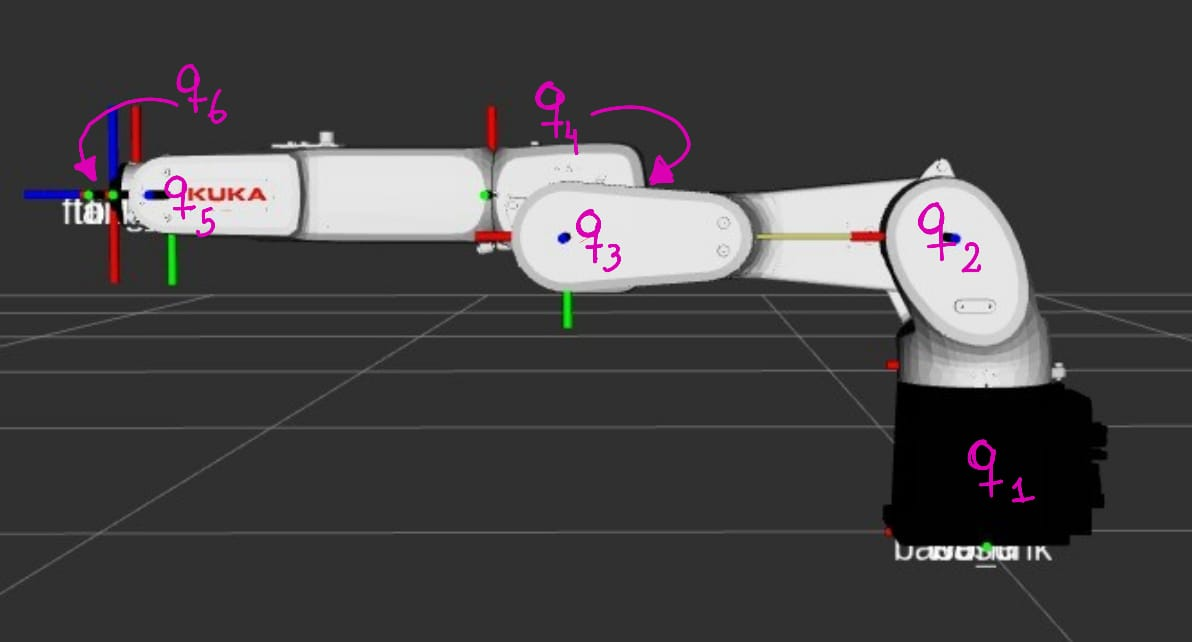
\includegraphics[width=0.95\columnwidth]{kuka_articulaciones.png}
    \caption{Robot KUKA KR 7 R900-3 y articulaciones consideradas.}
    \label{fig:robot_general}
\end{figure}

% ============================================================
\section{Asignación de marcos de referencia}

Para el desarrollo cinemático se definieron marcos de referencia
siguiendo la convención Denavit--Hartenberg estándar. Para cada
articulación revoluta, el eje $z_{i-1}$ se alineó con su eje de
rotación. El eje $x_i$ se seleccionó sobre la normal común entre
dos ejes $z$ consecutivos, mientras que el eje $y_i$ se obtuvo
aplicando la regla de la mano derecha.

Los marcos definidos mediante este procedimiento no coinciden
necesariamente con los marcos propios de los eslabones del URDF.
Por este motivo, el modelo URDF/XACRO se utiliza como referencia
geométrica y posteriormente como medio de validación del modelo
cinemático desarrollado.

\instr{Esta parte es obligatoria. Mostrar cómo se colocó cada marco antes de presentar la tabla DH. El eje $z_{i-1}$ debe asociarse con el eje de movimiento de la articulación correspondiente en la convención DH estándar. Explicar la elección de $x_i$ a partir de la normal común entre ejes consecutivos. El eje $y_i$ se obtiene mediante la regla de la mano derecha. Si se requieren marcos intermedios fijos, deben mostrarse y justificarse.}

Para cada marco se debe indicar:

\begin{itemize}
    \item origen $O_i$;
    \item orientación de $x_i$, $y_i$ y $z_i$;
    \item articulación asociada;
    \item relación geométrica con el marco anterior;
    \item cualquier desplazamiento fijo o corrección angular requerida por el modelo.
\end{itemize}

La asignación de marcos se realizó siguiendo la geometría de los
ejes articulares observada en el modelo URDF. Los marcos se
definieron de la siguiente manera:

\begin{itemize}
    \item \textbf{Marco $\{0\}$:} su origen $O_0$ se ubica sobre
    el eje de la primera articulación, en la base del robot.
    El eje $z_0$ coincide con el eje de rotación de $q_1$.

    \item \textbf{Marco $\{1\}$:} su origen $O_1$ se localiza
    sobre el eje de la segunda articulación. El eje $z_1$
    coincide con el eje de rotación de $q_2$ y $x_1$ se orienta
    sobre la normal común entre los ejes de $q_1$ y $q_2$.

    \item \textbf{Marco $\{2\}$:} el origen $O_2$ se sitúa sobre
    el eje de $q_3$. Debido a que los ejes de $q_2$ y $q_3$
    son paralelos, $x_2$ se escoge sobre la normal común entre
    ambos ejes y $z_2$ coincide con el eje de $q_3$.

    \item \textbf{Marco $\{3\}$:} su origen $O_3$ se establece
    sobre el eje de la cuarta articulación, en el punto alcanzado
    por la normal común entre los ejes de $q_3$ y $q_4$.
    El eje $z_3$ coincide con el eje de rotación de $q_4$.

    \item \textbf{Marco $\{4\}$:} se coloca en la intersección
    de los ejes de $q_4$ y $q_5$. El eje $z_4$ coincide con
    el eje de rotación de $q_5$.

    \item \textbf{Marco $\{5\}$:} se coloca en la intersección
    de los ejes de $q_5$ y $q_6$. El eje $z_5$ coincide con
    el eje de rotación de $q_6$.

    \item \textbf{Marco $\{6\}$:} corresponde al extremo de la
    cadena cinemática. La transformación fija entre el último
    eslabón y \texttt{tool0} se conserva de forma separada para
    representar correctamente el efector final.
\end{itemize}

En todos los casos, el eje $y_i$ se obtiene mediante la regla de
la mano derecha una vez definidos $x_i$ y $z_i$.

\begin{figure}[H]
    \centering
    \fbox{\parbox[c][5cm][c]{0.90\columnwidth}{\centering
    INSERTAR FIGURA PROPIA\\
    DEL ROBOT CON TODOS LOS FRAMES}}
    \caption{Asignación de marcos de referencia del robot KUKA KR 7 R900-3.}    \label{fig:frames}
\end{figure}

\subsection{Convención utilizada}

En este trabajo se utilizará la convención Denavit--Hartenberg
estándar para modelar la cinemática del robot KUKA KR 7 R900-3.
Bajo esta convención, cada transformación homogénea entre marcos
consecutivos se expresa mediante cuatro parámetros:
$\theta_i$, $d_i$, $a_i$ y $\alpha_i$.
La matriz homogénea elemental empleada es la correspondiente
a la formulación estándar de Denavit--Hartenberg.

\begin{equation}
A_{i-1}^{i} =
R_z(\theta_i)\,
T_z(d_i)\,
T_x(a_i)\,
R_x(\alpha_i).
\label{eq:dh_product}
\end{equation}

Su forma matricial es:

\begin{equation}
A_{i-1}^{i} =
\begin{bmatrix}
c_{\theta_i} & -s_{\theta_i}c_{\alpha_i} & s_{\theta_i}s_{\alpha_i} & a_i c_{\theta_i}\\
s_{\theta_i} & c_{\theta_i}c_{\alpha_i} & -c_{\theta_i}s_{\alpha_i} & a_i s_{\theta_i}\\
0 & s_{\alpha_i} & c_{\alpha_i} & d_i\\
0 & 0 & 0 & 1
\end{bmatrix}.
\label{eq:dh_matrix}
\end{equation}

donde $c_{\theta_i}=\cos\theta_i$ y $s_{\theta_i}=\sin\theta_i$.

\instr{Si el grupo decide utilizar DH modificado, debe cambiar explícitamente la ecuación, explicar la convención y mantenerla durante todo el informe. No se permite mezclar DH estándar y modificado sin justificación.}

% ============================================================
\section{Parámetros Denavit--Hartenberg}

\instr{Construir la tabla a partir de la geometría real del robot y del modelo URDF/XACRO. No copiar tablas de Internet sin verificar su correspondencia con los frames usados por el grupo. Todas las distancias deben expresarse en metros y los ángulos en radianes. Incluir offsets constantes dentro de $\theta_i$ cuando corresponda.}

\begin{table*}[t]
\centering
\caption{Parámetros Denavit--Hartenberg del robot \pendiente{MODELO}}
\label{tab:dh}
\renewcommand{\arraystretch}{1.25}
\begin{tabular}{cccccc}
\toprule
\textbf{Transformación} &
\textbf{$\theta_i$} &
\textbf{$d_i$ [m]} &
\textbf{$a_i$ [m]} &
\textbf{$\alpha_i$ [rad]} &
\textbf{Descripción} \\
\midrule
$A_0^1$ & \pendiente{$q_1+\cdots$} & \pendiente{...} & \pendiente{...} & \pendiente{...} & base $\rightarrow$ link 1 \\
$A_1^2$ & \pendiente{$q_2+\cdots$} & \pendiente{...} & \pendiente{...} & \pendiente{...} & link 1 $\rightarrow$ link 2 \\
$A_2^3$ & \pendiente{$q_3+\cdots$} & \pendiente{...} & \pendiente{...} & \pendiente{...} & link 2 $\rightarrow$ link 3 \\
$A_3^4$ & \pendiente{$q_4+\cdots$} & \pendiente{...} & \pendiente{...} & \pendiente{...} & link 3 $\rightarrow$ link 4 \\
$A_4^5$ & \pendiente{$q_5+\cdots$} & \pendiente{...} & \pendiente{...} & \pendiente{...} & link 4 $\rightarrow$ link 5 \\
$A_5^6$ & \pendiente{$q_6+\cdots$} & \pendiente{...} & \pendiente{...} & \pendiente{...} & link 5 $\rightarrow$ efector \\
\bottomrule
\end{tabular}
\end{table*}

\subsection{Verificación geométrica de los parámetros}

\instr{Explicar de dónde se obtuvo cada distancia y cada offset angular. Comparar, cuando sea posible, con dimensiones del URDF/XACRO o documentación oficial. Si existen transformaciones fijas adicionales, incluirlas como matrices separadas en lugar de ocultarlas.}

% ============================================================
\section{Cinemática directa}

La cinemática directa se obtiene mediante:

\begin{equation}
T_0^n =
A_0^1 A_1^2 \cdots A_{n-1}^{n}.
\label{eq:fk}
\end{equation}

Para un manipulador de seis grados de libertad:

\begin{equation}
T_0^6 =
A_0^1 A_1^2 A_2^3 A_3^4 A_4^5 A_5^6.
\end{equation}

La transformación final tiene la forma:

\begin{equation}
T_0^6 =
\begin{bmatrix}
R_0^6 & p_0^6 \\
0\;0\;0 & 1
\end{bmatrix},
\end{equation}

donde:

\begin{equation}
p_0^6 =
\begin{bmatrix}
x\\y\\z
\end{bmatrix},
\qquad
R_0^6 \in SO(3).
\end{equation}

\subsection{Matrices homogéneas individuales}

\instr{Escribir explícitamente todas las matrices $A_{i-1}^{i}$ después de sustituir los parámetros DH. Deben conservarse las variables articulares. No basta con pegar la matriz genérica. Si son demasiado extensas, pueden pasar expresiones auxiliares a un apéndice, pero las matrices fundamentales deben aparecer en el informe.}

\begin{equation}
A_0^1 =
\left[\begin{array}{cccc}
\color{red}\cdots & \color{red}\cdots & \color{red}\cdots & \color{red}\cdots\\
\color{red}\cdots & \color{red}\cdots & \color{red}\cdots & \color{red}\cdots\\
\color{red}\cdots & \color{red}\cdots & \color{red}\cdots & \color{red}\cdots\\
0 & 0 & 0 & 1
\end{array}\right]
\end{equation}

\begin{equation}
A_1^2 =
\left[\begin{array}{cccc}
\color{red}\cdots & \color{red}\cdots & \color{red}\cdots & \color{red}\cdots\\
\color{red}\cdots & \color{red}\cdots & \color{red}\cdots & \color{red}\cdots\\
\color{red}\cdots & \color{red}\cdots & \color{red}\cdots & \color{red}\cdots\\
0 & 0 & 0 & 1
\end{array}\right]
\end{equation}

\instr{Continuar hasta la última transformación.}

\subsection{Matriz de transformación total}

\instr{Presentar $T_0^6$ de manera simbólica o semisimbólica. Si la expansión completa es excesivamente larga, definir expresiones auxiliares, por ejemplo $c_{23}=\cos(q_2+q_3)$, e indicar claramente cómo se obtuvo.}

\begin{equation}
T_0^6 =
\textcolor{red}{\text{[RESULTADO DEL PRODUCTO MATRICIAL]}}.
\end{equation}

\subsection{Posición y orientación del efector}

Extraer:

\begin{equation}
p(q) =
\begin{bmatrix}
p_x(q)\\
p_y(q)\\
p_z(q)
\end{bmatrix}.
\end{equation}

\instr{Mostrar las expresiones finales de $p_x$, $p_y$ y $p_z$. Para la orientación, presentar la matriz de rotación $R_0^6$ y, adicionalmente, una representación interpretable: cuaternión o ángulos de Euler. Indicar la convención de Euler utilizada si corresponde.}

\subsection{Comprobaciones matemáticas}

La matriz de rotación debe cumplir aproximadamente:

\begin{align}
(R_0^6)^T R_0^6 &\approx I,\\
\det(R_0^6) &\approx 1.
\end{align}

\instr{Verificar estas propiedades al menos para una configuración numérica y mostrar el resultado. También comprobar que la última fila de toda transformación homogénea sea $[0\;0\;0\;1]$.}

% ============================================================
\section{Jacobiano del manipulador}

\instr{Para este parcial, el Jacobiano se utilizará principalmente para resolver la cinemática inversa de \textbf{posición}. El grupo debe obtenerlo a partir de su propio modelo cinemático. No basta con llamar una función externa sin explicar su formulación.}

Para una articulación revoluta, la contribución lineal puede obtenerse mediante:

\begin{equation}
J_{v_i} = z_{i-1} \times (o_n-o_{i-1}),
\end{equation}

donde $z_{i-1}$ es el eje de la articulación expresado en el marco base, $o_{i-1}$ es el origen del marco correspondiente y $o_n$ la posición del efector final.

Por tanto, para un manipulador de $n$ articulaciones se empleará el Jacobiano posicional:

\begin{equation}
J_v(q)=
\begin{bmatrix}
\dfrac{\partial p_x}{\partial q_1} & \cdots & \dfrac{\partial p_x}{\partial q_n}\\[6pt]
\dfrac{\partial p_y}{\partial q_1} & \cdots & \dfrac{\partial p_y}{\partial q_n}\\[6pt]
\dfrac{\partial p_z}{\partial q_1} & \cdots & \dfrac{\partial p_z}{\partial q_n}
\end{bmatrix}.
\end{equation}

\subsection{Jacobiano utilizado en el proyecto}

\instr{Presentar el Jacobiano posicional utilizado por el algoritmo de IK. Puede obtenerse analíticamente a partir de $p(q)$, geométricamente a partir de los frames o simbólicamente con SymPy, pero el informe debe mostrar de dónde sale.}

\begin{equation}
J_v(q)=\textcolor{red}{\text{[INSERTAR JACOBIANO POSICIONAL]}}.
\end{equation}

\subsection{Consideración de singularidades}

\instr{Explicar brevemente qué ocurre cuando el Jacobiano pierde rango o se encuentra cerca de una singularidad y cómo afecta esto al método iterativo. Para este primer parcial no se exige un estudio exhaustivo de singularidades.}

% ============================================================
\section{Cinemática inversa}

\subsection{Definición del problema}

Para este Primer Parcial Práctico, la cinemática inversa tendrá como objetivo obligatorio alcanzar una \textbf{posición cartesiana} deseada del efector final:

\begin{equation}
p_d =
\begin{bmatrix}
x_d\\
y_d\\
z_d
\end{bmatrix}.
\end{equation}

El algoritmo debe encontrar una configuración articular:

\begin{equation}
q^\star =
\begin{bmatrix}
q_1 & q_2 & \cdots & q_n
\end{bmatrix}^{T}
\end{equation}

tal que:

\begin{equation}
p(q^\star) \approx p_d.
\end{equation}

\instr{No se exige resolver orientación en la IK de este parcial. La orientación sí debe obtenerse en la cinemática directa a partir de $T_0^n$. Si algún grupo decide resolver pose completa como ampliación, debe documentar adicionalmente el error de orientación y el Jacobiano correspondiente.}

\subsection{Objetivo recibido mediante ROS 2}

El punto objetivo debe recibirse mediante el tópico:

\begin{center}
\texttt{/target}
\end{center}

utilizando el mensaje:

\begin{center}
\texttt{geometry\_msgs/msg/Point}.
\end{center}

Una prueba debe poder enviarse desde terminal mediante un comando equivalente a:

\begin{lstlisting}[language=bash]
ros2 topic pub /target geometry_msgs/msg/Point \
"{x: 0.40, y: 0.20, z: 0.50}" --once
\end{lstlisting}

\instr{Los valores del ejemplo son únicamente ilustrativos. Cada grupo debe escoger objetivos alcanzables para su robot y documentar los valores utilizados en sus pruebas.}

\subsection{Método numérico iterativo}

A partir de la cinemática directa, se define el error de posición en la iteración $k$:

\begin{equation}
e_k =
p_d - p(q_k).
\end{equation}

El Jacobiano posicional se evalúa en la configuración actual:

\begin{equation}
J_k = J_v(q_k).
\end{equation}

La actualización articular puede realizarse mediante la pseudoinversa:

\begin{equation}
q_{k+1}
=
q_k + \alpha J_k^{+} e_k,
\label{eq:ik_pinv}
\end{equation}

donde $\alpha$ es el factor de actualización y $J_k^{+}$ es la pseudoinversa del Jacobiano.

Cuando corresponda y sea matemáticamente válida, puede expresarse como:

\begin{equation}
J^{+}=J^T(JJ^T)^{-1}.
\end{equation}

\instr{Si se utiliza \texttt{numpy.linalg.pinv}, debe explicarse que corresponde al cálculo numérico de la pseudoinversa. No se exige implementar Damped Least Squares en este primer parcial; puede utilizarse únicamente como ampliación si el grupo desea estudiar comportamiento cercano a singularidades.}

\subsection{Configuración inicial}

El algoritmo debe partir de una configuración:

\begin{equation}
q_0 =
\begin{bmatrix}
q_{1,0} & q_{2,0} & \cdots & q_{n,0}
\end{bmatrix}^{T}.
\end{equation}

\instr{Documentar los valores iniciales utilizados. Deben corresponder a una configuración válida del robot y respetar sus límites articulares. Puede utilizarse una configuración home, el estado actual del robot o una semilla razonable elegida por el grupo.}

\subsection{Articulaciones utilizadas}

\instr{El grupo debe indicar qué articulaciones intervienen en la solución numérica. Si alguna articulación se mantiene fija durante la IK, debe indicarse su valor y justificarse. No asumir que todos los robots deben fijar las mismas articulaciones.}

\subsection{Límites articulares}

\instr{Presentar los límites de cada articulación utilizados por el algoritmo. Los valores deben provenir del URDF/XACRO o de documentación oficial. La solución final debe respetarlos.}

\begin{table}[H]
\centering
\caption{Límites articulares utilizados}
\begin{tabular}{ccc}
\toprule
\textbf{Joint} & \textbf{Mínimo [rad]} & \textbf{Máximo [rad]}\\
\midrule
$q_1$ & \pendiente{...} & \pendiente{...}\\
$q_2$ & \pendiente{...} & \pendiente{...}\\
$q_3$ & \pendiente{...} & \pendiente{...}\\
$q_4$ & \pendiente{...} & \pendiente{...}\\
$q_5$ & \pendiente{...} & \pendiente{...}\\
$q_6$ & \pendiente{...} & \pendiente{...}\\
\bottomrule
\end{tabular}
\end{table}

\subsection{Criterio de convergencia}

El error euclidiano de posición se define como:

\begin{equation}
e_p =
\|p_d-p(q_k)\|_2.
\end{equation}

El algoritmo se considera convergente cuando:

\begin{equation}
e_p < \varepsilon
\end{equation}

antes de alcanzar el número máximo de iteraciones.

\instr{El grupo debe indicar el valor de $\varepsilon$, el factor $\alpha$, el máximo de iteraciones y cualquier criterio adicional utilizado.}

\subsection{Publicación de la solución articular}

Una vez obtenida la solución $q^\star$, el nodo de cinemática inversa debe publicar los valores articulares en:

\begin{center}
\texttt{/joint\_states}
\end{center}

mediante mensajes:

\begin{center}
\texttt{sensor\_msgs/msg/JointState}.
\end{center}

Esto permite que \texttt{robot\_state\_publisher} actualice la configuración del robot y que el resultado sea visible en RViz2.

\instr{Los nombres y el orden de las articulaciones publicados deben coincidir con los definidos por el modelo URDF/XACRO del robot.}

\subsection{Verificación mediante cinemática directa}

La solución obtenida por IK debe verificarse nuevamente mediante la cinemática directa:

\begin{equation}
p_f = p(q^\star),
\end{equation}

y comprobar:

\begin{equation}
\|p_d-p_f\|_2 < \varepsilon.
\end{equation}

\instr{El nodo de FK debe permitir comprobar numéricamente la posición alcanzada. En la ejecución deben mostrarse, como mínimo, el objetivo solicitado, la posición final calculada y el error obtenido.}

% ============================================================
\section{Implementación en Python y ROS 2}

\subsection{Herramientas}

La implementación debe ser compatible con:

\begin{itemize}
    \item Ubuntu 24.04;
    \item ROS 2 Jazzy;
    \item Python 3;
    \item RViz2;
    \item \texttt{robot\_state\_publisher};
    \item \texttt{joint\_state\_publisher\_gui};
    \item NumPy y/o SymPy;
    \item SciPy, únicamente si el grupo la utiliza y la declara como dependencia.
\end{itemize}

\subsection{Nodo de cinemática directa}

\instr{Crear un nodo propio, por ejemplo \texttt{fk\_node.py}, que se suscriba a \texttt{/joint\_states} y calcule la transformación $T_0^n$ utilizando las matrices DH desarrolladas por el grupo. No debe limitarse a consultar TF y presentar ese resultado como si fuera su cinemática directa. TF puede utilizarse únicamente como referencia de validación.}

El nodo debe, como mínimo:

\begin{enumerate}
    \item suscribirse a \texttt{/joint\_states};
    \item leer y ordenar correctamente las articulaciones del robot;
    \item evaluar las matrices DH;
    \item calcular $T_0^n$;
    \item obtener la posición $(x,y,z)$;
    \item obtener la orientación del efector final, por ejemplo como cuaternión;
    \item mostrar los resultados de forma clara en consola.
\end{enumerate}

\instr{Publicar adicionalmente la pose como \texttt{PoseStamped} es válido, pero no es requisito obligatorio de este primer parcial. Sí es obligatorio calcular posición y orientación en FK.}

\subsection{Nodo de cinemática inversa}

\instr{Crear un nodo propio, por ejemplo \texttt{ik\_node.py}, que se suscriba obligatoriamente a \texttt{/target} con mensajes \texttt{geometry\_msgs/msg/Point}, resuelva la IK de posición y publique la solución articular en \texttt{/joint\_states}.}

El flujo mínimo esperado es:

\begin{verbatim}
/target  (Point: x,y,z)
       |
       v
    ik_node
       |
       v
/joint_states
       |
       +--> robot_state_publisher --> RViz2
       |
       +--> fk_node --> verificacion numerica
\end{verbatim}

El nodo de IK debe reportar:

\begin{itemize}
    \item objetivo recibido $(x_d,y_d,z_d)$;
    \item configuración inicial $q_0$;
    \item solución articular obtenida $q^\star$;
    \item número de iteraciones;
    \item posición alcanzada;
    \item error final;
    \item indicación clara de convergencia o no convergencia.
\end{itemize}

\subsection{Interacción con Joint State Publisher GUI}

\instr{El Joint State Publisher GUI también publica \texttt{/joint\_states}. Para mover manualmente el robot y probar FK puede utilizarse normalmente. Para las pruebas en las que \texttt{ik\_node.py} publique la solución en \texttt{/joint\_states}, no deben mantenerse dos publishers de estados articulares controlando simultáneamente el robot. El grupo debe cerrar el GUI durante esa prueba o documentar una arquitectura equivalente que evite el conflicto.}

% ============================================================
\section{Workspace ROS 2}

\subsection{Estructura mínima}

\instr{Mostrar la estructura real del workspace del grupo. No incluir \texttt{build/}, \texttt{install/} ni \texttt{log/} dentro del repositorio GitHub.}

\begin{lstlisting}
grupo_XX_robot_ws/
|-- src/
|   |-- grupoXX_robot_bringup/
|   |   |-- launch/
|   |   |   `-- display.launch.py
|   |   |-- package.xml
|   |   `-- setup.py / CMakeLists.txt
|   |
|   `-- grupoXX_robot_kinematics/
|       |-- grupoXX_robot_kinematics/
|       |   |-- fk_node.py
|       |   `-- ik_node.py
|       |-- resource/
|       |-- package.xml
|       |-- setup.py
|       `-- setup.cfg
|
|-- dependencias.repos
|-- instalar.sh
|-- entorno.sh
|-- README.md
|-- requirements.txt
`-- .gitignore
\end{lstlisting}

\instr{El paquete de descripción oficial del fabricante puede obtenerse mediante \texttt{dependencias.repos} o mediante el script de instalación. No es necesario duplicar repositorios externos completos dentro de GitHub. Es preferible declarar su URL y fijar una rama, tag o commit conocido.}

\subsection{Compilación}

Desde la raíz del workspace:

\begin{lstlisting}[language=bash]
source /opt/ros/jazzy/setup.bash
export RMW_IMPLEMENTATION=rmw_cyclonedds_cpp

rosdep install --from-paths src --ignore-src -r -y

colcon build --symlink-install
source install/setup.bash
\end{lstlisting}

\subsection{Ejecución del robot}

\begin{lstlisting}[language=bash]
ros2 launch grupoXX_robot_bringup display.launch.py
\end{lstlisting}

\subsection{Ejecución de los nodos propios}

Terminal para cinemática directa:

\begin{lstlisting}[language=bash]
ros2 run grupoXX_robot_kinematics fk_node
\end{lstlisting}

Terminal para cinemática inversa:

\begin{lstlisting}[language=bash]
ros2 run grupoXX_robot_kinematics ik_node
\end{lstlisting}

En otra terminal se envía un objetivo:

\begin{lstlisting}[language=bash]
ros2 topic pub /target geometry_msgs/msg/Point \
"{x: 0.40, y: 0.20, z: 0.50}" --once
\end{lstlisting}

\instr{Reemplazar los nombres anteriores por los nombres reales del paquete y ejecutables del grupo. Los valores del punto son de ejemplo. Todos los comandos del informe deben poder copiarse y ejecutarse.}

% ============================================================
\section{Validación de la cinemática directa}

\instr{Realizar al menos tres casos de prueba dentro de los límites articulares. Debe existir al menos una configuración no trivial. Evitar validar únicamente con todos los ángulos en cero.}

\begin{table*}[t]
\centering
\caption{Validación de la cinemática directa}
\label{tab:fk_validation}
\begin{tabular}{cccccc}
\toprule
\textbf{Caso} &
\textbf{$q$ [rad]} &
\textbf{$p_{calc}$ [m]} &
\textbf{$p_{ROS}$ [m]} &
\textbf{Error pos. [m]} &
\textbf{Error ori. [rad]} \\
\midrule
1 & \pendiente{...} & \pendiente{...} & \pendiente{...} & \pendiente{...} & \pendiente{...} \\
2 & \pendiente{...} & \pendiente{...} & \pendiente{...} & \pendiente{...} & \pendiente{...} \\
3 & \pendiente{...} & \pendiente{...} & \pendiente{...} & \pendiente{...} & \pendiente{...} \\
\bottomrule
\end{tabular}
\end{table*}

El error de posición se calculará como:

\begin{equation}
e_p =
\|p_{\text{calc}}-p_{\text{ref}}\|_2.
\end{equation}

\instr{Explicar qué se utiliza como referencia: TF del modelo, una medición obtenida del modelo oficial, o una verificación equivalente. RViz2 por sí solo es una visualización; la comparación numérica debe provenir de datos reproducibles.}

\subsection{Pruebas por transformaciones parciales}

\instr{Se recomienda validar la cadena de manera incremental, especialmente cuando existe un error de frames. Por ejemplo: $A_0^1$, $A_0^1A_1^2$, $A_0^1A_1^2A_2^3$, etc. Incluir capturas o resultados de los eslabones relevantes.}

% ============================================================
\section{Validación de la cinemática inversa}

\instr{Realizar al menos tres objetivos cartesianos alcanzables enviados mediante \texttt{/target}. Para cada caso mostrar $(x_d,y_d,z_d)$, configuración inicial, solución articular, posición final alcanzada, número de iteraciones y error final. Si el algoritmo no converge en un caso, documentarlo en vez de ocultarlo.}

\begin{table*}[t]
\centering
\caption{Pruebas de cinemática inversa}
\label{tab:ik_validation}
\begin{tabular}{cccccc}
\toprule
\textbf{Caso} &
\textbf{$p_d=[x_d,y_d,z_d]$} &
\textbf{$q_0$} &
\textbf{$q^\star$} &
\textbf{Iteraciones} &
\textbf{Error final [m]} \\
\midrule
1 & \pendiente{...} & \pendiente{...} & \pendiente{...} & \pendiente{...} & \pendiente{...} \\
2 & \pendiente{...} & \pendiente{...} & \pendiente{...} & \pendiente{...} & \pendiente{...} \\
3 & \pendiente{...} & \pendiente{...} & \pendiente{...} & \pendiente{...} & \pendiente{...} \\
\bottomrule
\end{tabular}
\end{table*}

\begin{figure}[H]
    \centering
    \fbox{\parbox[c][4cm][c]{0.90\columnwidth}{\centering
    INSERTAR CAPTURAS DE VALIDACIÓN\\
    DE LA CINEMÁTICA INVERSA}}
    \caption{Validación de objetivos de cinemática inversa en RViz2.}
\end{figure}

% ============================================================
\section{Repositorio GitHub y reproducibilidad}

\instr{Esta sección es obligatoria. El repositorio debe permitir que otra persona clone el proyecto y lo ejecute en una computadora limpia con Ubuntu 24.04 y ROS 2 Jazzy siguiendo únicamente el README. El enlace debe estar disponible antes de la entrega. Si el repositorio es privado, el docente debe tener acceso antes del plazo.}

\subsection{Enlace}

\begin{itemize}
    \item Repositorio: \texttt{https://github.com/USUARIO/REPOSITORIO}
    \item Rama de entrega: \texttt{\pendiente{main}}
    \item Commit evaluado: \texttt{\pendiente{HASH DEL COMMIT FINAL}}
\end{itemize}

\subsection{Contenido mínimo del repositorio}

El repositorio debe incluir:

\begin{enumerate}
    \item \texttt{README.md} completo;
    \item código fuente de los paquetes ROS 2 desarrollados por el grupo;
    \item launch files propios;
    \item \texttt{package.xml}, \texttt{setup.py}/\texttt{CMakeLists.txt} y archivos necesarios para compilar;
    \item \texttt{dependencias.repos} o mecanismo equivalente para recuperar dependencias externas;
    \item \texttt{instalar.sh} o instrucciones reproducibles de instalación;
    \item \texttt{entorno.sh} si se requieren variables de entorno;
    \item \texttt{requirements.txt} si se utilizan dependencias Python adicionales;
    \item \texttt{.gitignore};
    \item carpeta \texttt{docs/} con el informe final en PDF;
    \item capturas o datos estrictamente necesarios para reproducir las pruebas.
\end{enumerate}

\subsection{Archivos que no deben subirse}

No deben versionarse:

\begin{lstlisting}
build/
install/
log/
__pycache__/
*.pyc
.vscode/
.idea/
\end{lstlisting}

\instr{No subir el workspace entero comprimido como sustituto del repositorio. GitHub debe contener los archivos fuente y la información necesaria para reconstruir el workspace.}

\subsection{Requisitos del README}

El \texttt{README.md} debe contener, como mínimo:

\begin{enumerate}
    \item nombre del proyecto, robot y autores;
    \item objetivo del trabajo;
    \item software y versiones requeridas;
    \item instrucciones de clonación;
    \item instalación de dependencias;
    \item recuperación del paquete oficial del robot;
    \item compilación con \texttt{colcon build --symlink-install};
    \item comando \texttt{source install/setup.bash};
    \item comando exacto para abrir RViz2;
    \item comando para ejecutar FK;
    \item comando para ejecutar IK;
    \item ejemplo concreto de una prueba;
    \item tópicos, servicios o parámetros utilizados;
    \item estructura del repositorio;
    \item errores conocidos o consideraciones particulares.
\end{enumerate}

\subsection{Procedimiento mínimo de reproducción}

Otra persona debe poder ejecutar:

\begin{lstlisting}[language=bash]
git clone https://github.com/USUARIO/REPOSITORIO.git
cd REPOSITORIO

chmod +x instalar.sh
./instalar.sh

source /opt/ros/jazzy/setup.bash
export RMW_IMPLEMENTATION=rmw_cyclonedds_cpp
source install/setup.bash

ros2 launch grupoXX_robot_bringup display.launch.py
\end{lstlisting}

y posteriormente:

\begin{lstlisting}[language=bash]
ros2 run grupoXX_robot_kinematics fk_node
ros2 run grupoXX_robot_kinematics ik_node
\end{lstlisting}

\instr{Si estos comandos no son suficientes para reproducir el proyecto, el README está incompleto. Todo paso manual adicional debe documentarse.}

\subsection{Dependencias externas reproducibles}

\instr{Las dependencias externas deben quedar fijadas a una rama estable, tag o commit conocido. No depender únicamente de ``la última versión'' de un repositorio, porque una actualización futura puede romper el proyecto.}

Ejemplo conceptual de \texttt{dependencias.repos}:

\begin{lstlisting}
repositories:
  robot_description:
    type: git
    url: https://github.com/ORGANIZACION/REPOSITORIO.git
    version: RAMA_TAG_O_COMMIT
\end{lstlisting}

Posteriormente:

\begin{lstlisting}[language=bash]
mkdir -p src
vcs import src < dependencias.repos
\end{lstlisting}

% ============================================================
\section{Resultados y discusión}

\instr{Comparar los resultados matemáticos con ROS 2. Analizar errores, dificultades de asignación de frames, sensibilidad de la IK a la semilla inicial, comportamiento cerca de singularidades y cualquier diferencia entre el modelo matemático y el URDF/XACRO. Evitar una sección puramente descriptiva.}

\pendiente{DESARROLLO DEL GRUPO.}

% ============================================================
\section{Conclusiones}

\instr{Redactar entre tres y cinco conclusiones técnicas. Deben responder qué se logró, qué se validó, qué limitaciones se encontraron y qué aprendió el grupo sobre DH, FK, Jacobiano, IK y ROS 2. No repetir literalmente el resumen.}

\begin{itemize}
    \item \pendiente{Conclusión 1.}
    \item \pendiente{Conclusión 2.}
    \item \pendiente{Conclusión 3.}
\end{itemize}

% ============================================================
\section{Referencias}

\instr{Incluir documentación oficial del fabricante, repositorio oficial del modelo ROS 2 y bibliografía utilizada para DH, FK, Jacobiano e IK. Utilizar un formato consistente.}

\begin{thebibliography}{00}

\bibitem{robot_docs}
KUKA,
``KR AGILUS -- KR 7 R900-3, documentación técnica del fabricante,''
KUKA Robotics, consultado el 4 de octubre de 2026.

\bibitem{robot_ros}
\pendiente{Organización},
``\pendiente{Repositorio ROS 2 oficial o utilizado},''
GitHub, \pendiente{URL y commit/tag utilizado}.

\bibitem{robotics_book}
\pendiente{Autor},
\textit{\pendiente{Título del libro o recurso de robótica}},
\pendiente{Editorial/año}.

\end{thebibliography}

% ============================================================
\appendices

\section{Checklist previo a la entrega}

\begin{itemize}
    \item[$\square$] Todos los autores y el robot están correctamente identificados.
    \item[$\square$] Los frames aparecen en una figura propia.
    \item[$\square$] La tabla DH coincide con las matrices utilizadas.
    \item[$\square$] Se muestran todas las transformaciones necesarias.
    \item[$\square$] Se incluyen $p(q)$ y $R(q)$.
    \item[$\square$] Se presenta y explica el Jacobiano posicional.
    \item[$\square$] El nodo IK recibe el objetivo mediante \texttt{/target} (\texttt{Point}).
    \item[$\square$] El nodo IK publica la solución en \texttt{/joint\_states}.
    \item[$\square$] Se documentan $q_0$, tolerancia, límites e iteraciones.
    \item[$\square$] Hay al menos tres pruebas de FK.
    \item[$\square$] Hay al menos tres pruebas de IK.
    \item[$\square$] Los resultados numéricos se comparan con ROS 2.
    \item[$\square$] El repositorio GitHub es accesible.
    \item[$\square$] El README permite reproducir el proyecto desde cero.
    \item[$\square$] \texttt{build/}, \texttt{install/} y \texttt{log/} no están en GitHub.
    \item[$\square$] El commit final está indicado en el informe.
    \item[$\square$] Se eliminaron todos los textos \textcolor{red}{[PENDIENTES]} e instrucciones no requeridas.
\end{itemize}

\end{document}
